\documentclass[11pt]{report}
\title{Assignment 1: Genetic Algorithm for the Knapsack Problem}
\author{Guilherme Santos \texttt{fc62533}}
\date{\today}

\usepackage[left=1in,right=1in,top=1in,bottom=1in]{geometry}
\usepackage{tikz,pgfplots}
\usepackage{subfig}
\usepackage{caption}
\usepackage{amsmath}
\begin{document}

\maketitle

\section*{Parallelization Strategies Used}
My approach to parallelizing this problem was similar to the
'Embarrassingly Parallel Programming' exercises of the first week, where we divided the data, in this case the array of individuals, into chunks and processed each chunk on a separate thread.
By diving the data into smaller chunks, the workload can be distributed evenly across the cores, thereby ensuring that all cores are utilized effectively.
First, I parallelized the function \texttt{populateInitialPopulationRandomly()} and the \textit{'for loops'} that calculate the fitness, cross-over and mutation and noticed that the algorithm took longer to launch since \texttt{populateInitialPopulationRandomly()} ran faster in sequential mode than it did in parallel, 
so I decided to leave it in sequential mode.
There are functions, such as \texttt{tournament(int tournamentSize, Random r)} and \texttt{bestOfPopulation()}, whose parallelization I don't believe would be beneficial 
or possible since in \texttt{bestOfPopulation()} all the threads would need to access the entire array to find the best individual, 
and in \texttt{tournament(int tournamentSize, Random r)} the parallelization seems complex and has a high risk of introducing bugs.
The generations were not parallelized since each generation N requires generation N-1.

\section*{Results}

\begin{figure}[h]
  
  \caption*{Execution time with \texttt{N\_GENERATIONS = 500} and \texttt{POP\_SIZE=100000}}
 
  \begin{minipage}{0.5\textwidth}
    \centering
    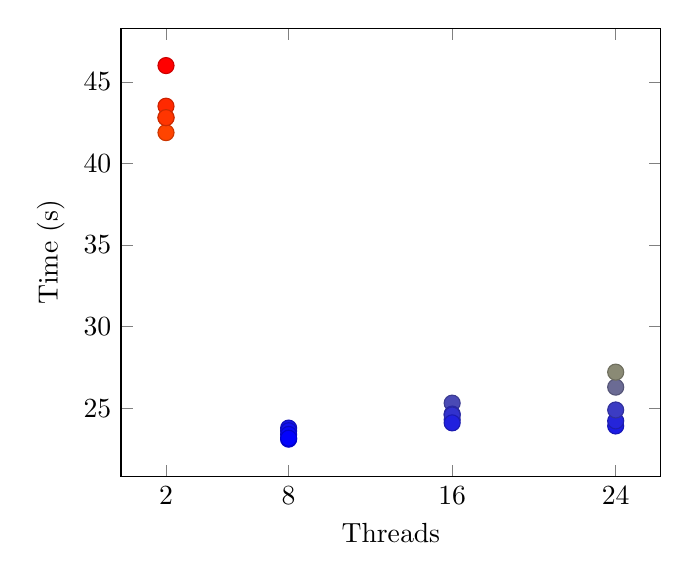
\begin{tikzpicture}
      \begin{axis}[xlabel={Threads}, ylabel={Time (s)}, xtick={2, 8, 16, 24}]
        \addplot+[only marks, scatter, mark size=2.9pt]
        coordinates {
          (2,41.89)
          (2,42.81)
          (2,46.00)
          (2,43.51)
          (2,42.81)
          (8,23.78)
          (8,23.62)
          (8,23.1)
          (8,23.39)
          (8,23.16)
          (16,25.31)
          (16,24.3)
          (16,24.64)
          (16,24.58)
          (16,24.1)
          (24,26.29) 
          (24,23.91) 
          (24,24.22) 
          (24,27.21) 
          (24,24.89)
        };
      \end{axis}
    \end{tikzpicture}
    
    \caption{Parallel}
  \end{minipage}%
  \hspace{2em}
  \begin{minipage}{0.5\textwidth}
    \centering
    \begin{tikzpicture}
      \begin{axis}[xlabel={Population ($10^5$)}, ylabel={Time (s)}, xtick={1}]
        \addplot+[only marks, scatter, mark size=2.9pt]
        coordinates {
          (1,69.36)
          (1,68.99)
          (1,72.20)
          (1,77.72)
          (1,73.91)
        };
      \end{axis}
    \end{tikzpicture}
    \caption{Sequential}
  \end{minipage}
  \end{figure}

  \vspace{-12pt}
  According to Figure 1, the best execution time was with 8 threads.  
  
  \vspace{12pt}
  The ideal chunk size is:
  $$chunkSize = \frac{POP\_SIZE}{\#Threads} = \frac{100000}{8} = 12500$$

  Inprovement in performance:


  $$SpeedUp = \frac{\overline{Sequential}}{\overline{Parallel}} = \frac{72.44s}{23.41s} \approx 3 $$
  
  \vspace{12pt}

  As a result, we can say that the parallel version is 3 times faster than the sequential one.
  
\section*{The Mann-Whitney U test}

\begin{figure}[h]
  \centering
  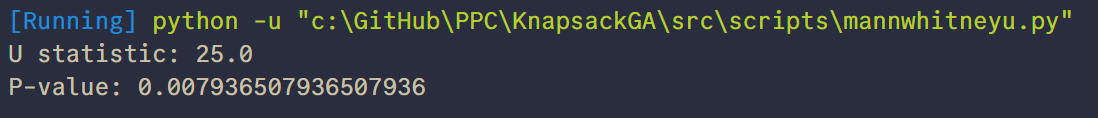
\includegraphics[width=0.7\textwidth]{script.png}
  \caption{Script's output}
  
\end{figure}

The p-value is small (less than 0.05) so we can conclude that the difference between 
the execution times is statistically significant and not due to random chance.
\section*{Environment}
\begin{tabular}{|c|c|c|c|c|c|}
  \hline
  CPU & Cores & Threads & RAM &  Operating System & Java\\
  \hline
  Intel Core i7-13700 & 16 & 24 & 32GB 6000MHz & Windows 11 & 21\\
  \hline
\end{tabular}


\end{document}
